\section{Verified preliminary evidence}
\label{sec:evidence}
The following results come from completed development experiments. They
constrain method design; they are not evidence that the pending candidate
has succeeded. The source manifest and generated tables accompany this draft.

\subsection{A stronger training baseline}
\begin{table}[t]
\centering\small
\caption{Completed anchor evidence: two-seed means on custom synthetic and paired ND development data. Historical rows differ in training; only the two R41 raw forms are a matched FP32 parameterization comparison.}
\label{tab:anchors}
\begin{tabular}{lrrrr}
\toprule
Anchor/output & SYN PSNR & SYN $E_{\rm temp}$ & ND PSNR & ND $E_{\rm temp}$\\
\midrule
Dynamic synthetic (R34) & 26.234 & 10.505 & 23.453 & 3.166\\
Fixed mixed Slim (R40) & 25.134 & 11.363 & 24.861 & 3.628\\
Matched Slim FP32 (R41) & 25.131 & 11.362 & 24.861 & 3.627\\
Expanded FP32 (R41) & 26.186 & 10.007 & 25.847 & 3.630\\
Expanded + finite & 26.394 & 7.286 & 25.734 & 2.804\\
Expanded + recursive & 26.503 & 6.520 & 25.758 & 2.553\\
Earlier native training (R26) & -- & -- & 27.138 & 3.313\\
\bottomrule
\end{tabular}
\end{table}

Table~\ref{tab:anchors} separates historical anchors from the matched
training-form comparison. In the matched FP32 experiment, restoring MBR/BN
training improves synthetic raw PSNR over direct Slim fine-tuning by
0.968 and 1.142\,dB for the two seeds. The corresponding paired-real gains
are 0.171 and 1.799\,dB. Both deploy to the same 4,075-parameter spatial
class. Training parameterization is therefore a material baseline choice.
This is known spatial reparameterization, not a new video mechanism.

The expanded control uses 49,978 training parameters, including an inactive
frozen warm head; 47,239 parameters are optimized. It is a controlled
fine-tuning study, not a complete reproduction of the official warm-up,
loss, and long-schedule training. To preserve the pretrained numerical
starting function, the wide raw convolution executes its preserved and
additional output blocks separately. This retains its parameters and
mathematical operator but differs from the upstream single wide-kernel call.

The domain trade-off remains important. Expanded training approximately
recovers the synthetic quality of the dynamic-synthetic anchor while
improving its paired-real mapping. It still trails the earlier native
training reference in paired-real PSNR. Those historical training schemes
differ in several respects and do not isolate one causal factor.
No single online model is obtained by taking the best weight separately
for each domain.

\begin{figure}[t]
\centering
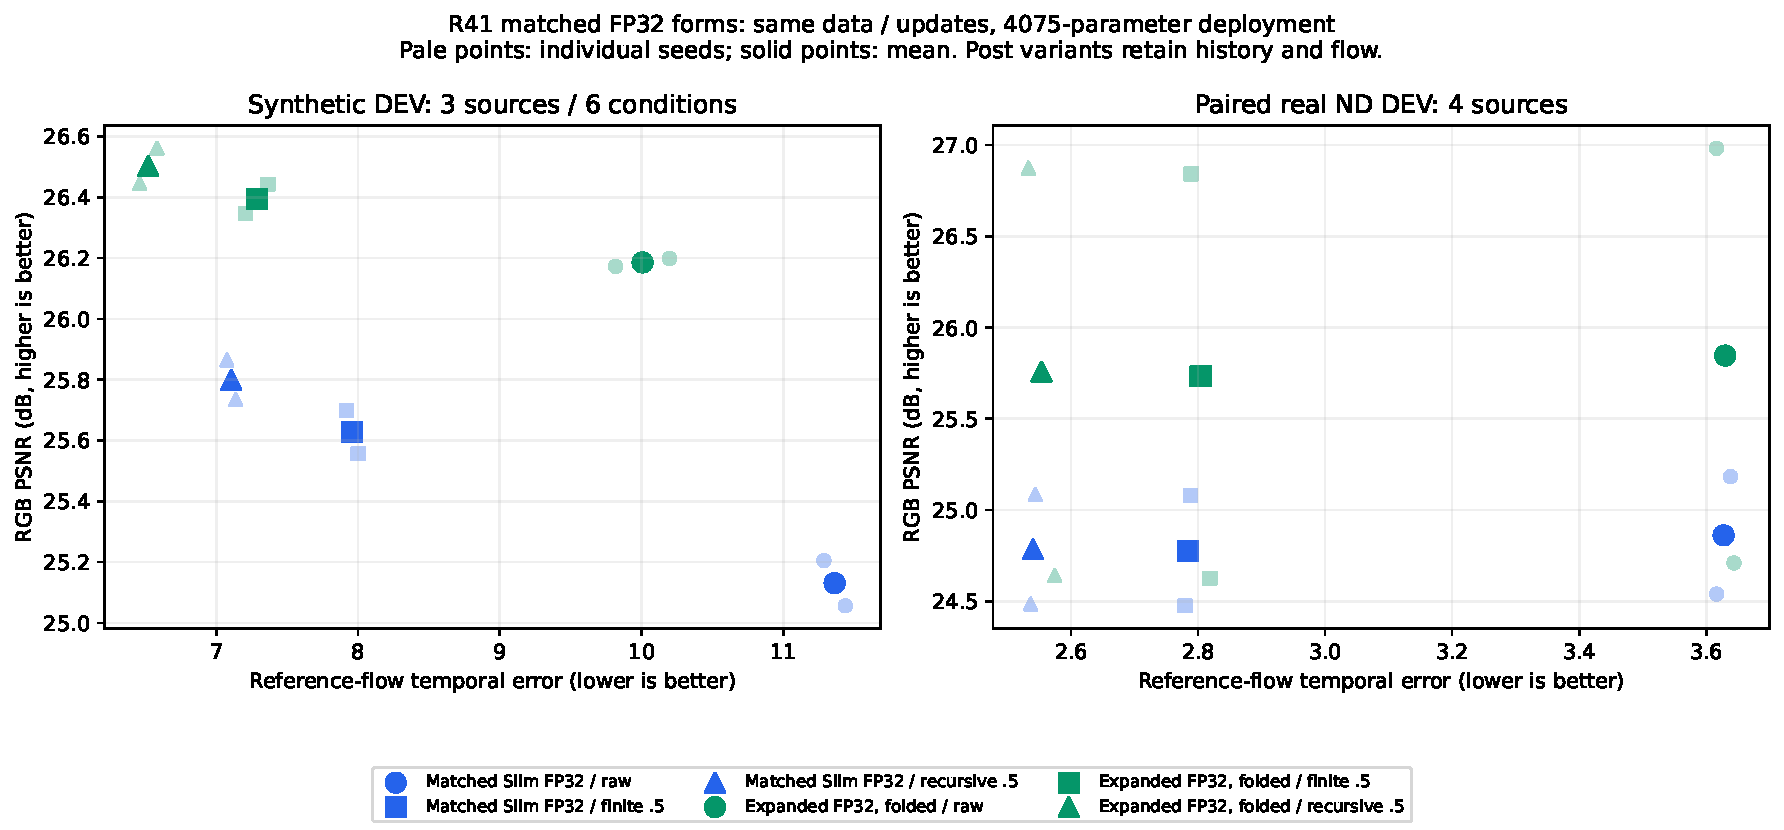
\includegraphics[width=\linewidth]{matched_forms.pdf}
\caption{Completed matched FP32 training-form comparison. Pale points retain
both individual seeds; solid points are their means. The real-domain spread
and the quality--temporal trade-off are visible. Postprocessed outputs use
motion and history; they are not stateless predictions.}
\label{fig:forms}
\end{figure}

Mean improvement does not imply reliable per-clip improvement. On paired-real
video 121, expanded seed 0 loses 2.606\,dB against its matched Slim control
and shows sky colour bias in the fixed-frame inspection. Its four-source
real mean is 24.710\,dB, versus 26.983\,dB for expanded seed 1. Raw
paired-real temporal error is not consistently reduced. All source/seed
pairs and all four metrics remain part of the record.

\subsection{Classical recursion is a necessary reference}
\begin{table}[t]
\centering\small
\caption{Classical references on the same R34 weights. Quality uses the full synthetic pilot. Resident CPU timing uses only the first 16 bear/P20 frames at $480\times854$, two Torch threads and one OpenCV thread. Ranges are run-average extrema, not confidence intervals or phone timings.}
\label{tab:classical}
\begin{tabular}{lrrrr}
\toprule
Output & PSNR & $E_{\rm temp}$ & History MiB & CPU ms/frame [range]\\
\midrule
Raw & 26.234 & 10.505 & 0.000 & 100.9 [80.9, 106.5]\\
Finite .5 & 26.466 & 7.543 & 4.691 & 184.1 [168.1, 188.5]\\
Recursive .5 & 26.610 & 6.735 & 9.382 & 186.5 [179.6, 192.5]\\
\bottomrule
\end{tabular}
\end{table}

On the same strong dynamic-synthetic anchor, recursive fusion improves
the finite reference's quality and temporal error
(Table~\ref{tab:classical}). Its persistent fused output is a meaningful
information advantage, not a negligible implementation detail. The
recursive reference cannot be replaced by a weaker two-frame average
when judging a proposed temporal model.

The measured CPU ranges overlap, so the small difference between the finite
and recursive medians is not established as a significant speed difference.
These timings concern the stated R34 weights and workload; they are not
measurements of the later expanded anchor or the pending rational model.
The extra stored RGB history and motion work remain part of deployment.

\subsection{Fixed local statistics do not rescue this anchor}
\begin{table}[t]
\centering\small
\caption{Fixed known TLC192 versus the same R41 expanded weights. No retraining or window search.}
\label{tab:tlc}
\begin{tabular}{llrr}
\toprule
Domain & Seed & Raw $\Delta$PSNR & Raw temporal ratio\\
\midrule
Synthetic & 0 & -0.305 & 1.0114\\
Synthetic & 1 & -0.415 & 1.0082\\
Paired ND & 0 & -2.312 & 1.0416\\
Paired ND & 1 & -2.343 & 1.0268\\
\bottomrule
\end{tabular}
\end{table}

The fixed TLC~\cite{tlc} control replaces only the channel-pooling node
with exact local averaging at a window of 192 pixels. Both development
domains and both seeds lose raw PSNR; the paired-real temporal ratios also
exceed the registered 1.02 upper bound (Table~\ref{tab:tlc}).
Across the 20 raw seed--condition pairs, five PSNR deltas are positive,
but all eight paired-real deltas are negative. The worst paired-real
condition loses 3.716\,dB.

The fixed instance and its local window search are stopped. This result
does not prove that all local aggregation or global-statistic adaptations
are ineffective. It also does not justify a speed claim: localizing the
channel map adds approximately 0.299 convolution GMAC at $1080\mathrm p$,
with prefix sums and memory traffic additional to that count.

\subsection{Pending candidate results}
\pending{The R44 factorial is still running at this manuscript snapshot.
Its raw, finite, recursive, per-condition, and per-seed final results must
be inserted only after both complete budgets and deployment-export gates
finish normally. No current loss curve or intermediate checkpoint supplies
this missing evidence.}
